%%%%%%%%%%%%%%%%%%%%%%%%%%%%%%%%%%%%%%%%%%%%%%%%%%%
%
%  New template code for TAMU Theses and Dissertations starting Fall 2012.  
%  For more info about this template or the 
%  TAMU LaTeX User's Group, see http://www.howdy.me/.
%
%  Author: Wendy Lynn Turner 
%	 Version 1.0 
%  Last updated 8/5/2012
%
%%%%%%%%%%%%%%%%%%%%%%%%%%%%%%%%%%%%%%%%%%%%%%%%%%%
%%%                           APPENDIX - Chapter 3
%%%%%%%%%%%%%%%%%%%%%%%%%%%%%%%%%%%%%%%%%%%%%%%%%%%

\phantomsection
\chapter{\uppercase{Addendum to Section \ref{sec::BF}}}
\label{sec::appendix_BF}

%%%%%%%%%%%%%%%%%%%%%%%%%%%%%%%%%%%%%%%%%%%%%%%%%%%
%%%   Section - Limits of the Linear Polygonal Basis Functions
\section{Limits of the Linear Polygonal Basis Functions}
\label{sec::appendix_BF_Limits}

As it was stated in Section \ref{sec::BF_2DLinear}, the Wachspress, mean value, and maximum entropy coordinates are all undefined on the boundary of the polygonal element. 

\begin{figure}[hbt]
\centering
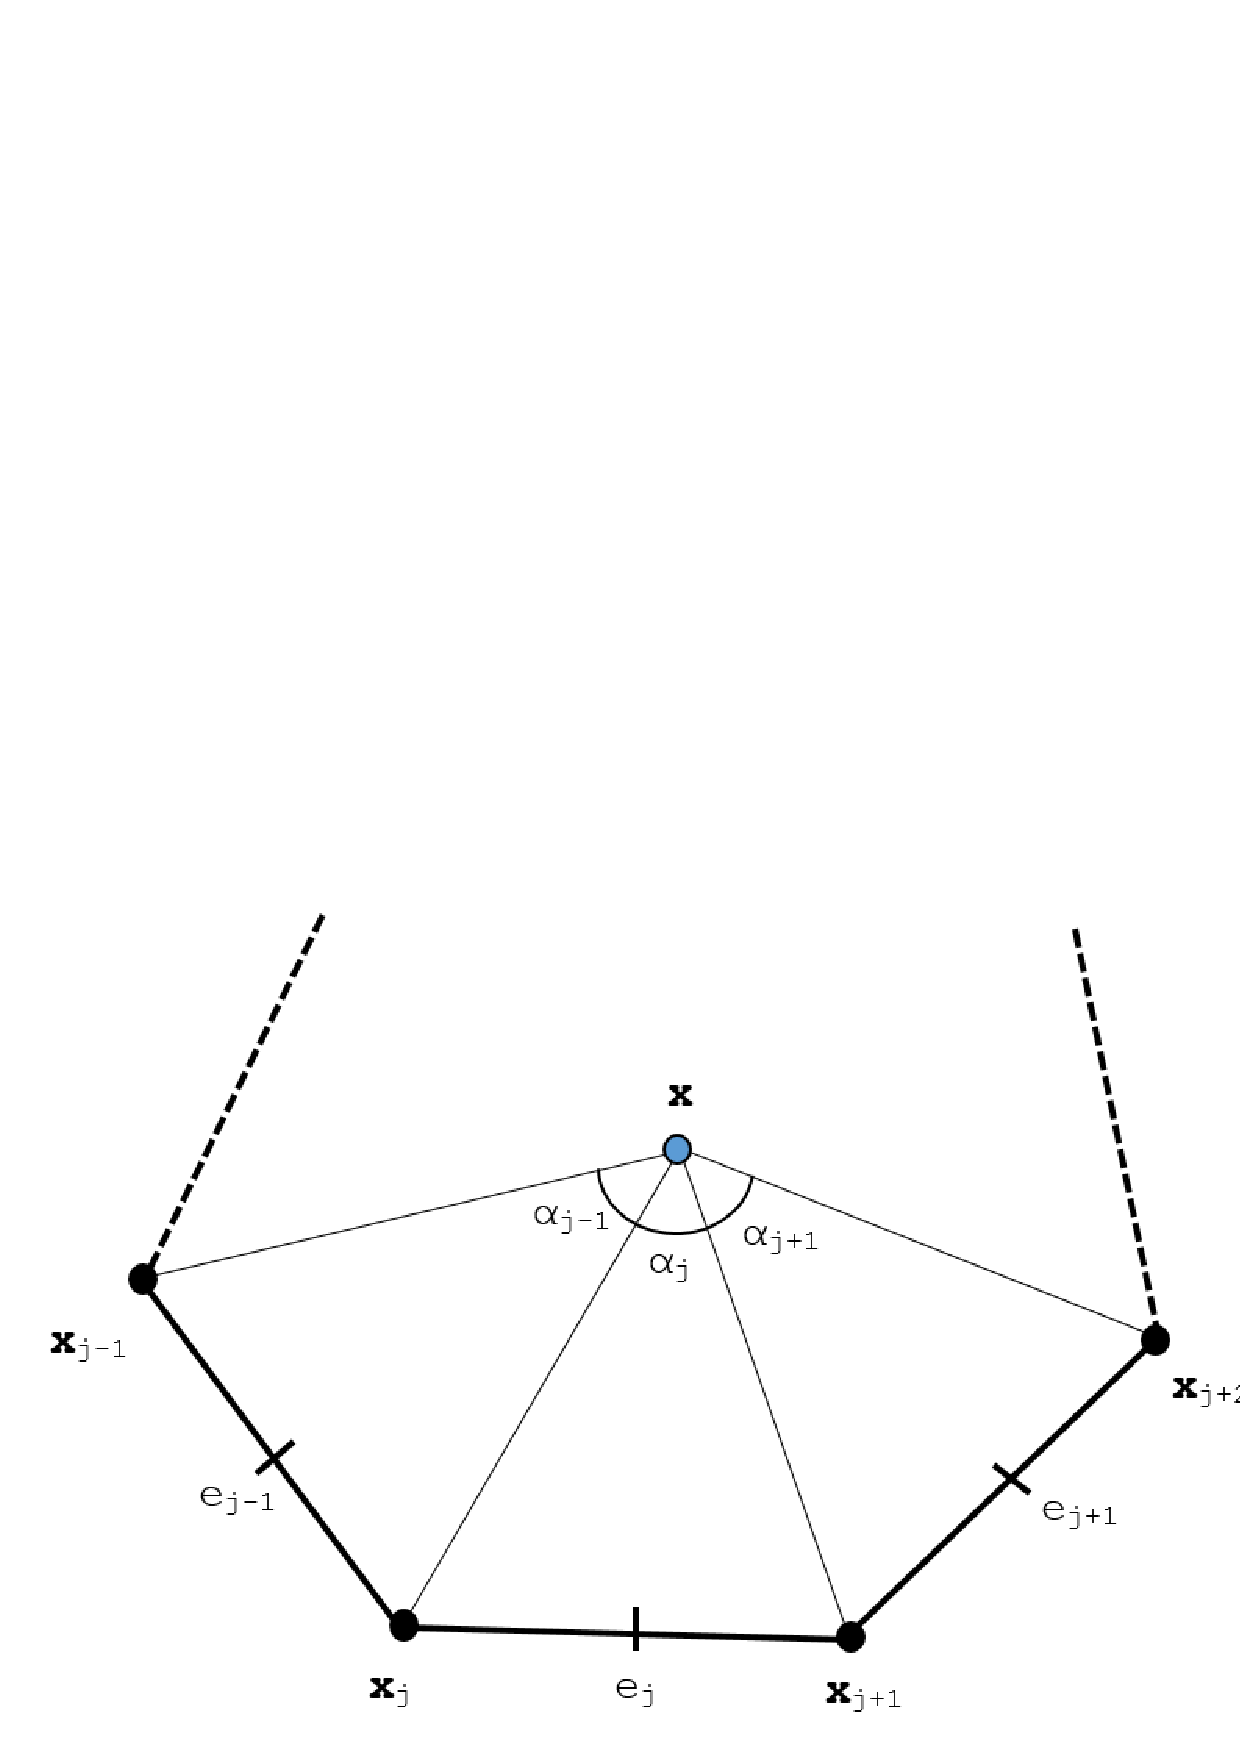
\includegraphics[width=0.65\textwidth]{figures/appendices/ref_polygon.png}
\caption{Arbitrary polygon with geometric properties used for 2D basis function generation.}
\label{fig::App_BF_2D_ref_polygon}
\end{figure}

%%%%%%%%%%%%%%%%%%%%%%%%%%%%%%%%%%%%%%%%%%%%%%%%%%%
%%%  Sub Section - Wachspress Limits
\subsection{Limits of the Wachspress Coordinates}
\label{sec::appendix_BF_Limits_Wachspress}

\begin{equation}
\label{eq::App_BF_WachBF}
\lambda_i^{W} (\vec{x}) = \frac{w_i^W  (\vec{x}) }{\sum_j w_j^W  (\vec{x}) }
\end{equation}

\noindent where the weight function for vertex $i$, $w_i$, has the following definition:

\begin{equation}
\label{eq::BF_wach_weights}
w_i (\vec{x})  = \frac{A(\vec{x}_{i-1}, \vec{x}_{i}, \vec{x}_{i+1})}{A(\vec{x}, \vec{x}_{i-1}, \vec{x}_{i}) \, A(\vec{x}, \vec{x}_{i}, \vec{x}_{i+1})}
\end{equation}

%%%%%%%%%%%%%%%%%%%%%%%%%%%%%%%%%%%%%%%%%%%%%%%%%%%
%%%  Sub Section - MV Limits
\subsection{Limits of the Mean Value Coordinates}
\label{sec::appendix_BF_Limits_MV}

\begin{equation}
\label{eq::App_BF_MVBF}
\lambda_i^{MV} (\vec{x}) = \frac{w_i^{MV}  (\vec{x}) }{\sum_j w_j^{MV}  (\vec{x}) }
\end{equation}

\noindent where the weight function for vertex $i$, $w_i$, has the following definition:

\begin{equation}
\label{eq::BF_MV_weights}
w_i (\vec{x})  = \frac{\tan(\alpha_{i-1} / 2) + \tan(\alpha_i / 2)}{|\vec{x}_i - \vec{x}|}
\end{equation}

%%%%%%%%%%%%%%%%%%%%%%%%%%%%%%%%%%%%%%%%%%%%%%%%%%%
%%%  Sub Section - ME Limits
\subsection{Limits of the Maximum Entropy Coordinates}
\label{sec::appendix_BF_Limits_ME}


\begin{equation}
\label{eq::App_BF_MEBF}
\lambda_i^{ME} (\vec{x}) = \frac{w_i^{ME}  (\vec{x}) }{\sum_j w_j^{ME}  (\vec{x}) }
\end{equation}

\noindent where the weight function for vertex $i$, $w_i$, has the following definition:

\begin{equation}
\label{eq::BF_ME_weights}
w_i (\vec{x})  = m_i(\vec{x}) \exp(-  \kappa \cdot (\vec{x}_i - \vec{x}))
\end{equation}

%%%%%%%%%%%%%%%%%%%%%%%%%%%%%%%%%%%%%%%%%%%%%%%%%%%
%%%   Section - Analytical 2D PWL Integration
\section{Analytical Integration of the 2D PWL Basis Functions}
\label{sec::appendix_BF_PWL2}

In Section \ref{sec::BF_2DLinear_PWL}, we provided the functional form for the Piecewise Linear (PWL) coordinates. We noted that of the linearly-complete 2D polygonal coordinates, PWL is the only one that can perform analytical integrations of the elementary matrices. We now describe the procedures to perform these analytical integrations of the elementary matrices.


\begin{equation}
\label{eq::2D_tri_ref_BF}
\begin{aligned}
	b_1(r,s) & = 1-r-s \\
	b_2(r,s) & = r \\
	b_3(r,s) & = s 
\end{aligned}
\end{equation}

%%%%%%%%%%%%%%%%%%%%%%%%%%%%%%%%%%%%%%%%%%%%%%%%%%%
%%%   Section - Analytical PWQ
\section{Analytical Form for the Quadratic Serendipity PWL Basis Functions}
\label{sec::appendix_BF_PWQ}

%%%%%%%%%%%%%%%%%%%%%%%%%%%%%%%%%%%%%%%%%%%%%%%%%%%
%%%   Section - Analytical 3D PWL Integration
\section{Analytical Integration of the 3D PWL Basis Functions}
\label{sec::appendix_BF_PWL3}



\begin{equation}
\label{eq::3D_tetref_BF}
\begin{aligned}
	b_1(r,s,t) & = 1-r-s-t \\
	b_2(r,s,t) & = r \\
	b_3(r,s,t) & = s \\
	b_4(r,s,t) & = t
\end{aligned}
\end{equation}
